\question Draw an example of each of the following situations \newline
{\tabulinesep=1mm
\begin{tabu}{|p{5cm} | p{5cm}| p{5cm}|}
\hline
One to one AND NOT onto (injective but not surjective) & Onto 
AND NOT one to one (surjective but not injective) & One to one 
AND onto (bijection, i.e. injective AND surjective)\\  
\hline
\begin{solution}[1 in] .\newline 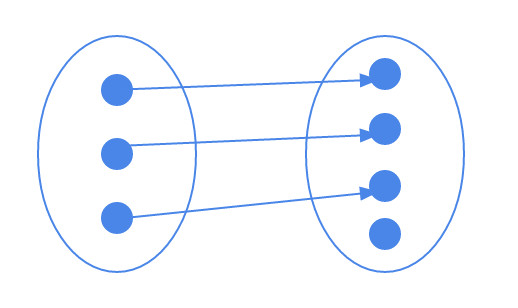
\includegraphics[width=4.5cm, height=30mm]{draw_injection.jpg} 
\end{solution} &  \begin{solution}[1 in] .\newline  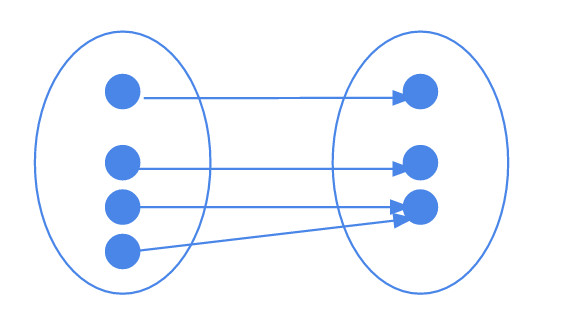
\includegraphics[width=4.5cm, height=30mm]{draw_surjection.jpg} \end{solution} &  \begin{solution}[1 in] .\newline 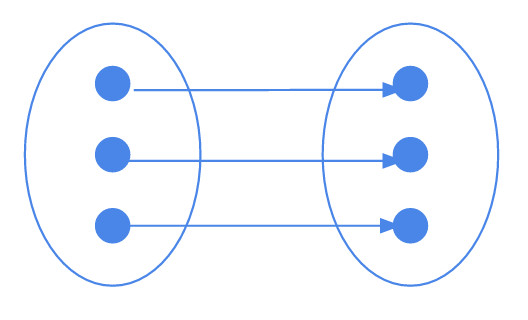
\includegraphics[width=4.5cm, height=30mm]{draw_bijection.jpg} \end{solution} \\
\hline
\end{tabu}
}